\documentclass[a4paper,11pt]{z}

%\usepackage[ngerman]{babel}
% use mac coding
%\usepackage[applemac]{inputenc}
%cite "`author ,year""
\usepackage{latexsym}
\usepackage{natbib,amsmath}
\usepackage{bm}
% neue Rechtschreibung, AMSMath, AMSSymb, A4 Format
\usepackage{amsmath,amssymb,a4wide}
%Grafiken, Zeilenabstand
\usepackage{graphicx, setspace}
 \usepackage{fancyhdr, fancybox}
 \usepackage[leqno,fleqn,intlimits]{empheq}
%Bookmarks, Hyperlinks
%\usepackage[bookmarks=true, bookmarksopen=true,
%            bookmarksnumbered=true, colorlinks,citecolor = black,filecolor = black,
%            linkcolor = black,urlcolor  = black,plainpages=false,hyperindex=true]{hyperref}
%index
\usepackage{makeidx}
%pfad zu sweave package
%\usepackage{/Library/Frameworks/R.framework/Resources/share/texmf/Sweave}
% pdf einstellungen
%\hypersetup{
%       pdftitle={},
%       pdfauthor={Robert Ferstl, Josef Hayden},
%       pdfsubject={Inhalt},
%        pdfkeywords={}
%        pdfcreator={},
%       pdfproducer={}
%     }
%Absatzabstaende
%\setlength{\parindent}{0.0cm} \setlength{\parskip}{1.5ex plus 0.5ex minus 0.5ex}
%Zeilenabstand in Tabellen
%\renewcommand{\arraystretch}{2}

%\pagestyle{headings}

\usepackage{natbib}


\usepackage{listings}
\usepackage{color}


\title{termstrc: A Package for Term Structure Estimation with R}


\author{Robert Ferstl\hspace{0.5cm}Josef Hayden}

\Abstract{
Zero-coupon yield curves and credit spread curves are important inputs for various financial models, e.g. pricing of securities, risk management, monetary policy issues. Since zero-coupon rates are rarely directly observable, they have to be estimated from market data for existing coupon bonds. The literature broadly distinguishes between parametric and spline-based methods. We implement two widely-used term structure estimation procedures, i.e. the parametric Nelson and Siegel approach and the Svensson approach.

Moreover, we implement the traditional way of credit spread calculation, where individually estimated zero-coupon yield curves are substracted from a risk-free reference curve. Goodness-of-fit tests are provided to compare the results of the different estimation methods. We illustrate the usage of our functions by practical examples with data from European and CEE government bonds, and European corporate bonds.
}

\Keywords{term structure, interest rates,  \proglang{R}}
\Plainkeywords{term structure, interest rates, R} %% without formatting

 %Index
\makeindex

\begin{document}

%define colors for syntax highlighting
\definecolor{darkblue}{rgb}{0,0,.5}
\definecolor{darkred}{rgb}{0.4,0.0,0}
\definecolor{commentcolor}{rgb}{0,0.5,0.25}
\definecolor{stringcolor}{rgb}{0.5,0.0,0}

\definecolor{myblue}{rgb}{.8, .8, 1}
\newcommand*\mybluebox[1]{%
\colorbox{myblue}{\hspace{1em}#1\hspace{1em}}}

\lstdefinelanguage{R}%
  {keywords={abbreviate,abline,abs,acos,acosh,action,add1,add,%
      aggregate,alias,Alias,alist,all,anova,any,aov,aperm,append,apply,%
      approx,approxfun,apropos,Arg,args,array,arrows,as,asin,asinh,%
      atan,atan2,atanh,attach,attr,attributes,autoload,autoloader,ave,%
      axis,backsolve,barplot,basename,besselI,besselJ,besselK,besselY,%
      beta,binomial,body,box,boxplot,break,browser,bug,builtins,bxp,by,byrow,%
      c,C,call,Call,case,cat,category,cbind,ceiling,character,char,%
      charmatch,check,chol,chol2inv,choose,chull,class,close,cm,codes,%
      coef,coefficients,co,col,colnames,colors,colours,commandArgs,%
      comment,complete,complex,conflicts,Conj,contents,contour,%
      contrasts,contr,helmert,contrib,convolve,cooks,coords,%
      distance,coplot,cor,cos,cosh,count,fields,cov,covratio,wt,CRAN,%
      create,crossprod,cummax,cummin,cumprod,cumsum,curve,cut,cycle,D,%
      data,dataentry,date,dbeta,dbinom,dcauchy,dchisq,de,debug,%
      debugger,Defunct,default,delay,delete,deltat,demo,de,density,%
      deparse,dependencies,Deprecated,deriv,description,detach,%
      dev2bitmap,dev,cur,deviance,off,prev,,dexp,df,dfbetas,dffits,%
      dgamma,dgeom,dget,dhyper,diag,diff,digamma,dim,dimnames,dir,%
      dirname,dlnorm,dlogis,dnbinom,dnchisq,dnorm,do,dotplot,double,%
      download,dpois,dput,drop,drop1,dsignrank,dt,dummy,dump,dunif,%
      duplicated,dweibull,dwilcox,dyn,edit,eff,effects,eigen,else,%
      emacs,end,environment,env,erase,eval,equal,evalq,example,exists,%
      exit,exp,expand,expression,External,extract,extractAIC,factor,%
      fail,family,fft,file,filled,find,fitted,fivenum,fix,floor,for,%
      For,formals,format,formatC,formula,Fortran,forwardsolve,frame,%
      frequency,ftable,ftable2table,function,gamma,Gamma,gammaCody,%
      gaussian,gc,gcinfo,gctorture,get,getenv,geterrmessage,getOption,%
      getwd,gl,glm,globalenv,gnome,GNOME,graphics,gray,grep,grey,grid,%
      gsub,hasTsp,hat,heat,help,hist,home,hsv,httpclient,I,identify,if,%
      ifelse,Im,image,\%in\%,index,influence,measures,inherits,install,%
      installed,integer,interaction,interactive,Internal,intersect,%
      inverse,invisible,IQR,is,jitter,kappa,kronecker,labels,lapply,%
      layout,lbeta,lchoose,lcm,legend,length,levels,lgamma,library,%
      licence,license,lines,list,lm,load,local,locator,log,log10,log1p,%
      log2,logical,loglin,lower,lowess,ls,lsfit,lsf,ls,machine,Machine,%
      mad,mahalanobis,make,link,margin,match,Math,matlines,mat,matplot,%
      matpoints,matrix,max,mean,median,memory,menu,merge,methods,min,%
      missing,Mod,mode,model,response,mosaicplot,mtext,mvfft,na,nan,%
      names,omit,nargs,nchar,ncol,NCOL,new,next,NextMethod,nextn,%
      nlevels,nlm,noquote,NotYetImplemented,NotYetUsed,nrow,NROW,null,%
      numeric,\%o\%,objects,offset,old,on,Ops,optim,optimise,optimize,%
      options,or,order,ordered,outer,package,packages,page,pairlist,%
      pairs,palette,panel,par,parent,parse,paste,path,pbeta,pbinom,%
      pcauchy,pchisq,pentagamma,persp,pexp,pf,pgamma,pgeom,phyper,pico,%
      pictex,piechart,Platform,plnorm,plogis,plot,pmatch,pmax,pmin,%
      pnbinom,pnchisq,pnorm,points,poisson,poly,polygon,polyroot,pos,%
      postscript,power,ppoints,ppois,predict,preplot,pretty,Primitive,%
      print,prmatrix,proc,prod,profile,proj,prompt,prop,provide,%
      psignrank,ps,pt,ptukey,punif,pweibull,pwilcox,q,qbeta,qbinom,%
      qcauchy,qchisq,qexp,qf,qgamma,qgeom,qhyper,qlnorm,qlogis,qnbinom,%
      qnchisq,qnorm,qpois,qqline,qqnorm,qqplot,qr,Q,qty,qy,qsignrank,%
      qt,qtukey,quantile,quasi,quit,qunif,quote,qweibull,qwilcox,%
      rainbow,range,rank,rbeta,rbind,rbinom,rcauchy,rchisq,Re,read,csv,%
      csv2,fwf,readline,socket,real,Recall,rect,reformulate,regexpr,%
      relevel,remove,rep,repeat,replace,replications,report,require,%
      resid,residuals,restart,return,rev,rexp,rf,rgamma,rgb,rgeom,R,%
      rhyper,rle,rlnorm,rlogis,rm,rnbinom,RNGkind,rnorm,round,row,%
      rownames,rowsum,rpois,rsignrank,rstandard,rstudent,rt,rug,runif,%
      rweibull,rwilcox,sample,sapply,save,scale,scan,scan,screen,sd,se,%
      search,searchpaths,segments,seq,sequence,setdiff,setequal,set,%
      setwd,show,sign,signif,sin,single,sinh,sink,solve,sort,source,%
      spline,splinefun,split,sqrt,stars,start,stat,stem,step,stop,%
      storage,str,strstrheight,stripplot,strsplit,structure,strwidth,sub,%
      subset,substitute,substr,substring,sum,summary,sunflowerplot,svd,%
      sweep,switch,symbol,symbols,symnum,sys,status,system,t,table,%
      tabulate,tan,tanh,tapply,tempfile,terms,terrain,tetragamma,text,%
      time,title,topo,trace,traceback,transform,tri,trigamma,trunc,try,%
      ts,tsp,typeof,unclass,undebug,undoc,union,unique,uniroot,unix,%
      unlink,unlist,unname,untrace,update,upper,url,UseMethod,var,%
      variable,vector,Version,vi,warning,warnings,weighted,%
      which,while,window,write,\%x\%,x11,X11,xedit,xemacs,xinch,xor,%
      xpdrows,xy,xyinch,yinch,zapsmall,zip},%
   otherkeywords={!,!=,~,$,*,\&,\%/\%,\%*\%,\%\%,<-,<<-,_,/},%
   alsoother={._$},%
   sensitive,%
   morecomment=[l]\#,%
   morestring=[d]",%
   morestring=[d]'% 2001 Robert Denham
  }

%settings for R syntaxhighlighting
\lstset{basicstyle=\ttfamily\small,
keywordstyle=\bfseries\color{darkblue},
stringstyle=\ttfamily,
showstringspaces=false,
language=R,
identifierstyle=,
commentstyle=\color{commentcolor},
stringstyle=\color{stringcolor}}


  \maketitle

%  \abstract{
%Zero-coupon yield curves and credit spread curves are important inputs for various financial models, e.g. pricing of securities, risk management, monetary policy issues. Since zero-coupon rates are rarely directly observable, they have to be estimated from market data for existing coupon bonds. The literature broadly distinguishes between parametric and spline-based methods. We implement two widely-used term structure estimation procedures, i.e. the parametric Nelson and Siegel approach and the Svensson approach.
%
%Moreover, we implement the traditional way of credit spread calculation, where individually estimated zero-coupon yield curves are substracted from a risk-free reference curve. Goodness-of-fit tests are provided to compare the results of the different estimation methods. We illustrate the usage of our functions by practical examples with data from European and CEE government bonds, and European corporate bonds.
%}
  \section{Introduction}

The \proglang{R} package \pkg{termstrc} consists of methods for estimating the term structure of interest rates from market data.

In this section we provide the basic concepts of bond pricing which are required for the estimation of the term structure of interest rates. Section 2 explains the ideas behind the two used models. Details about the notation and the optimisation procedure are presented in section 3. Section 4 includes a complete step-by-step example.


Since zero-coupon rates are rarely directly observable, they have to be estimated from market data for existing coupon bonds. For a coupon bond the following information is typically observable on the market: the maturity date $m$ , the clean price $p_c$ and the cashflows $c_t$ (coupons and redemption payment) which occur at $t=1,...n$. An investor who wants to buy the bond has to pay the dirty price $p_d$ which consists of the quoted market price (clean price) $p_c$ and the accrued interest $a$.

The term structure of interest rates can usually be described in three ways: the discount function, the
spot rate function and the forward rate function.

The bond pricing equation under continuous compounding is the present value of all cashflows.

\begin{equation}
  \label{bondpriceeq}
  p_c+a = \sum_{t=1}^n \ c_t e^{-s_tm_t}
\end{equation}

The spot rate $s_t$ is the yield-to maturity for a $t$-period zero-coupon bond. $m_t$ is the time to maturity of the $t$-th cash flow. A plot of the yields against times to maturity produces the zero-coupon yield curve.

The yield-to-maturity is the solution for $y$ in the following equation.

\begin{equation}
  \label{yield}
  p_c+a=\sum_{t=1}^n \ c_t e^{-ym_t}
\end{equation}

An equivalent formulation of the bond price equation makes use of the discount factors $d_t=\delta(m_t)=e^{-s_tm_t}$. The continuous discount function $\delta(\cdot)$ is formed by interpolation of the discount factors.

\begin{equation}
  \label{bondprceq2}
  p_c+a=\sum_{t=1}^n \ c_t \delta(m_t) \end{equation}


The implied $j$-period forward rate is calculated as

\begin{equation}
  \label{forwrate}
  f_{t|j}=\frac{js_j-ts_t}{j-t}=s_j+(s_j-s_t)\frac{t}{j-t}
\end{equation}

The instantaneous forward at the time $t$ equals

\begin{equation}
  \label{instfwdrate}
  f_t=\lim_{\Delta t \rightarrow 0}=\left[s_{t+\Delta t}+(s_{t+\Delta t}-s_t)\frac{t}{\Delta t}\right]=s_t+t\frac{\partial s}{\partial t}
\end{equation}

The spot rate is the integral of the instantaneous forward rate.


 \section{The Nelson/Siegel and Svensson method}

\label{nels-svenss-meth}

Assuming that a function between the spot rates and the maturities exists, we can estimate the term structure of interest rates. \cite{Nelson1987} proposed a parsimonious model of the yield curve. They model the forward rate with a second order differential equation.

\bigskip
\ovalbox{
\begin{minipage}{410pt}
\begin{equation}\label{nsfwd}
    f(m,\bm{b}) = \beta_0 + \beta_1\exp\left(-\frac{m}{\tau_1}\right)
    +\beta_2\frac{m}{\tau_1}\exp\left(-\frac{m}{\tau_1}\right)
    %\frac{1-\exp(-\frac{m}{\tau_1})}{\frac{m}{\tau_1}} + %\beta_2\left(\frac{1-\exp(-\frac{m}{\tau_1})}{\frac{m}{\tau_1}} - %\exp(-\frac{m}{\tau_1})\right)
\end{equation}
\end{minipage}
}
\bigskip

The corresponding spot rate curve is as follows.

\bigskip
\ovalbox{
\begin{minipage}{410pt}
\begin{equation}\label{nsspot}
    s(m,\bm{b}) = \beta_0 + \beta_1\frac{1-\exp(-\frac{m}{\tau_1})}{\frac{m}{\tau_1}} + \beta_2\left(\frac{1-\exp(-\frac{m}{\tau_1})}{\frac{m}{\tau_1}} - \exp(-\frac{m}{\tau_1})\right)
\end{equation}
\end{minipage}
}
\bigskip

The choice of the parameters ${\bm{b}} = \left(\beta_0,\beta_1,\beta_2,\tau_1\right)$ enables us to construct various possible shapes of the spot rate and the instantaneous  forward rate curve. The constant term $\beta_0$ is the limit of the  instantaneous forward rate when the time to maturity tends to infinity. The first exponential term $\beta_1 \exp(-\frac{m}{\tau_1})$ can be interpreted as a short-term contribution. It will decrease monotonically to zero with time to maturity when $\beta_1$ is positive. The second exponential term $\beta_2 \frac{m}{\tau_1} \exp(-\frac{m}{\tau_1})$ generates a hump-shape, which is realized in the medium term, because it starts at zero and decays to zero.

The following code replicates figure 2 on page 477 in \cite{Nelson1987}, see Figure 1.

\begin{lstlisting}[frame=leftline]
m <- seq(0,10,0.01)     # time to maturity

beta_1 <- 1             # parameters
tau_1 <- 1
beta_2 <- 1
beta_0 <- 1

par(lwd=2)

# beta_1
plot(m,beta_1*exp(-m/tau_1),type="l",col=1,
     xlab="Time to maturity",
     ylab="Model curves",ylim=c(0,2.1),lty=4)

# beta_2
lines(m,beta_2*(m/tau_1)*exp(-m/tau_1),lty=2,col=2)

# forward rate curve
lines(m,beta_0+beta_1*exp(-m/tau_1)+beta_2*(m/tau_1)*exp(-m/tau_1),col=3)

abline(h=1,lty=3,col=4)

legend("topright",legend=c(expression(beta[1]*exp(-m/tau[1])),
       expression(beta[2]*(m/tau[1])*exp(-m/tau[1])),
       expression(beta[0]),
       expression(f(m,b))),
       lty=c(4,2,3,1), col=c(1,2,4,3))
\end{lstlisting}

\begin{figure}[h]
\label{fwdcurvenelson}
\centering
	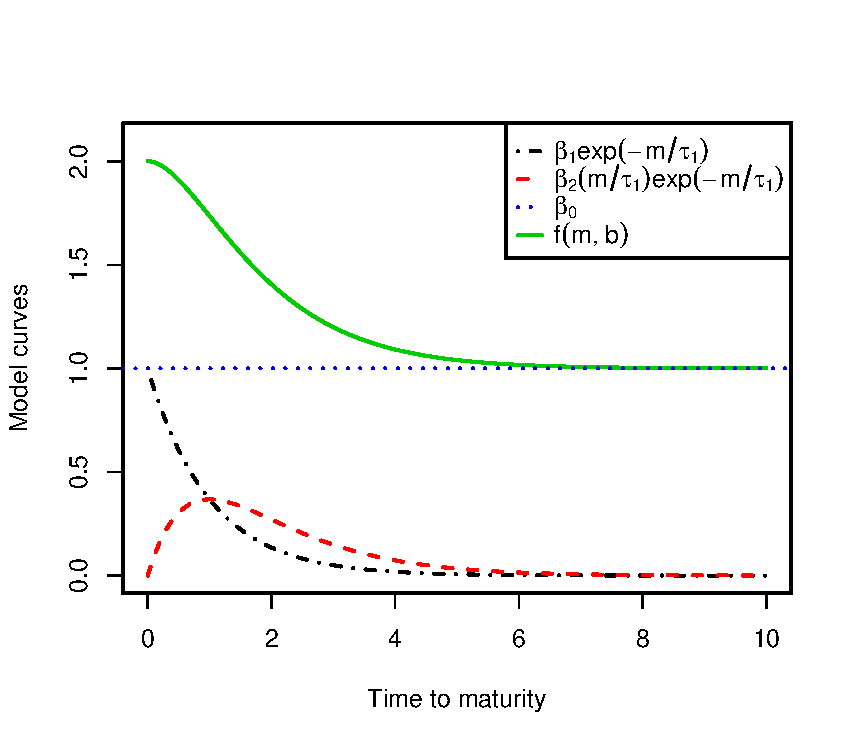
\includegraphics[width=0.80\textwidth]{pics/ns.pdf}
	\caption{Decomposition of the Nelson/Siegel forward rate function}
\end{figure}


\cite{Svensson1994} extended the functional form of the forward rate curve by two additional parameters which allows for a second hump-shape.

\bigskip
\ovalbox{
\begin{minipage}{410pt}
\begin{equation}\label{svfwd}
    f(m,\bm{b}) = \beta_0 + \beta_1\exp\left(-\frac{m}{\tau_1}\right)
    +\beta_2\frac{m}{\tau_1}\exp\left(-\frac{m}{\tau_1}\right)
    +\beta_3\frac{m}{\tau_2}\exp\left(-\frac{m}{\tau_2}\right)
\end{equation}
\end{minipage}
}
\bigskip

The spot rate is calculated as

\bigskip
\ovalbox{
\begin{minipage}{410pt}
\begin{multline}\label{svspot}
    s(m,\bm{b}) = \beta_0 + \beta_1\frac{1-\exp(-\frac{m}{\tau_1})}{\frac{m}{\tau_1}} + \beta_2\left(\frac{1-\exp(-\frac{m}{\tau_1})}{\frac{m}{\tau_1}} - \exp(-\frac{m}{\tau_1})\right) \\+ \beta_3\left(\frac{1-\exp(-\frac{m}{\tau_2})}{\frac{m}{\tau_2}} - \exp(-\frac{m}{\tau_2})\right),
\end{multline}
\end{minipage}
}
\bigskip

with a parameter vector ${\bm{b}} = \left(\beta_0,\beta_1,\beta_2,\tau_1,\beta_3,\tau_2\right)$.

The impact of the parameters can be described as follows \citep[see][p.7]{Bolder1999}:

\begin{itemize}
\item $\beta_0$ is the asymptotic value of the forward rate (spot rate) function.  The curve will tend towards the asymptote as the time to maturity approaches  $\infty$ ($\beta_0 >0$).
\item $\beta_1$ determines the starting (short-term) value of the curve in terms of deviation from the asymptote (the sum $\beta_0$ and $\beta_1$) is the vertical intercept. Moreover, it defines the basic speed with which the curve tends toward its long-term trend.
\item $\tau_1$ specifies the position of the first hump or the U-shape on the curve ($\tau_1>0$).
\item $\beta_2$ determines the magnitude and direction of the hump. If $\beta_2 >0$  a hump will occur at  $\tau_1$, whereas $\beta_2<0$, a U-shaped value will occur at $\tau_1$.
\item $\tau_2$ specifies the position of the second hump or the U-shape on the curve ($\tau_2>0$).
\item $\beta_3$ analogously  to  $\beta_2$ determines the magnitude and direction of the second hump.
\end{itemize}

The following code replicates figure 1 on page 8 in \cite{Bolder1999}. It shows the decomposition of the forward rate curve, see Figure 2.

\begin{lstlisting}[frame=leftline]
m <- seq(0,15,0.01)     # time to maturity

beta_1 <- 1             # parameters
tau_1 <- 1
beta_2 <- 1
beta_0 <- 1
tau_2 <-2
beta_3 <- 2


par(lwd=2)

# beta_1
plot(m,beta_1*exp(-m/tau_1),type="l",col=1,
     xlab="Time to maturity",
     ylab="Model curves",ylim=c(0,2.4),lty=4)

# beta_2
lines(m,beta_2*(m/tau_1)*exp(-m/tau_1),lty=2,col=2)

# beta_3
lines(m,beta_3*(m/tau_2)*exp(-m/tau_2),lty=6,col=6)

# forward rate curve
lines(m,beta_0+beta_1*exp(-m/tau_1)+beta_2*(m/tau_1)*exp(-m/tau_1) +
beta_3*(m/tau_2)*exp(-m/tau_2),col=3)

# beta_0
abline(h=1,lty=3,col=4)

legend("topright",legend=c(expression(beta[1]*e^(-m/tau[1])),
       expression(beta[2]*(m/tau[1])*e^(-m/tau[1])),
       expression(beta[0]),
       expression(beta[3]*(m/tau[2])*e^(-m/tau[2])),
       expression(f(m,b))),
       lty=c(4,2,3,6,1), col=c(1,2,4,6,3))
\end{lstlisting}

\begin{figure}[h]
\label{fwdcurve-sven}
\centering
	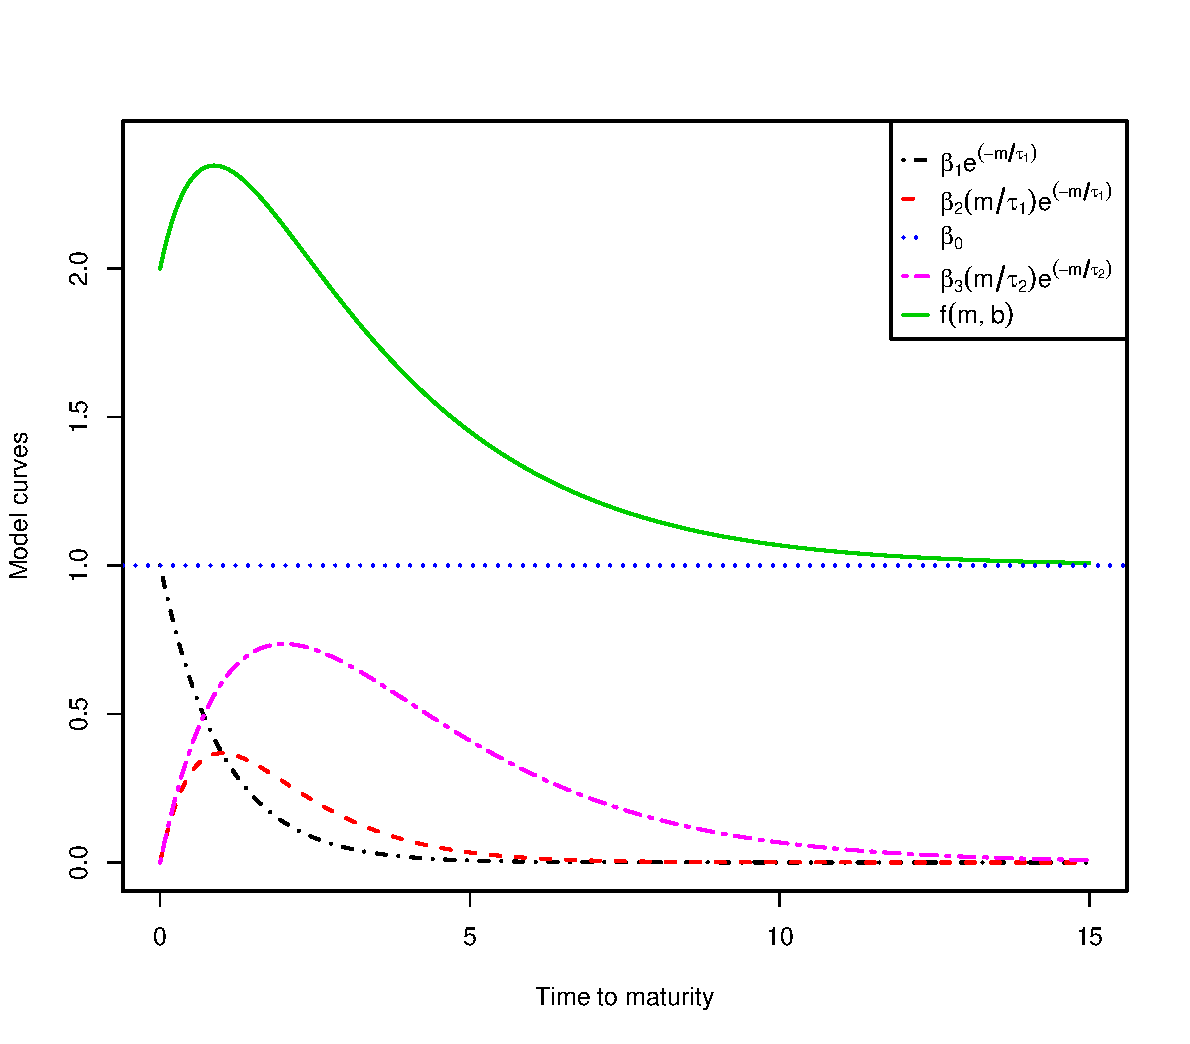
\includegraphics[width=0.80\textwidth]{pics/sv.pdf}
	\caption{Decomposition of the Svensson forward rate function}
\end{figure}


\subsection*{Credit-spread estimation}
The credit-spread estimation in the package \pkg{termstrc} is limited to the usual way of calculating a credit spread curve, i.e subtracting the yield-curve of a reference country $s_{ref}(\mathbf{m,b})$ from the yield-curves $s_j(\mathbf{m,b})$ of other countries .


\begin{equation}
cs_j(\mathbf{m}) = s_j(\mathbf{m,b}) - s_{ref}(\mathbf{m,b})
\end{equation}

\begin{tabular}{ll}
$cs_j(\mathbf{m})$ & credit-spread between country $j$ and reference country $ref$ \\
$s_j(\mathbf{m.b})$ &spot-rate curve of country $j$ with maturity vector  $\mathbf{m}$ \\
$s_{ref}(\mathbf{m,b})$ & spot-rate curve of the reference country
\end{tabular}

The spot-rate functions are defined as in equation (\ref{nsspot}) and (\ref{svspot}). For a more advanced method of credit-spread estimation see \citep{Jankowitsch2004}.

 \section{Estimation procedure}

%The objective is to construct zero-coupon yield curves based on observable data of coupon bonds. As  explained above, a theoretical bond price can be estimated using the basic bond characteristics, which are quoted at the market. Therefore the challenge of the optimisation is to minimize the deviation of the theoretical from the dirty price. The following explanations provide an insight in how the estimation problem may be structured. Moreover, we attach importance to an easy translation of the theoretical problem to a practical implementation. Thus we use a matrix notation to explain the estimation procedure for an approach that estimates the yield curves for one group of bonds, e.g. country, rating class.

In this section we describe in detail the optimisation problem which has to solved when estimating the term structure of interest rates from market data.

\subsection{Notation}

\subsubsection*{Maturity matrix $\bm{M}$}

\begin{equation}\label{maturitym}
\bm{M}_{\left[n\times m\right]} = \{m_{ij}\}
\end{equation}

The number of rows $n$ is determined through the number of cashflows of the bond $j$ with the longest maturity. For each bond $j$ exists a column with the corresponding cashflow dates. Dates after the maturity of the bond $j$ are filled up with zeros till the maturity date of the bond with the longest maturity. One element $m_{ij}$ of the matrix  refers, therefore, to the maturity date of  the $i$-th cashflow of the $j$-th bond.

\subsubsection*{Cashflow matrix $\bm{C}$}

 \begin{equation}\label{cashflowm}
\bm{C}_{\left[n\times m\right]} = \{c_{ij}\}
\end{equation}

 The cashflow matrix is defined analogously to the maturity matrix.  One element $c_{ij}$  of the matrix refers to the cashflow of the $i$-th cashflow of the $j$-th bond. Note, that the last cashflow of a each bond includes the redemption payment.

\subsubsection*{Discount factor matrix $\bm{D}$}

 \begin{equation}\label{discountm}
\bm{D}_{\left[n\times m\right]} = \{d_{ij}\}
\end{equation}

 The discount factor matrix is also defined analogously to the maturity matrix. One element $d_{ij}$ of the matrix refers to the discount factor associated with  the $i$-th cashflow of the $j$-th bond. An individual discount factor $d_{ij}$ is constructed as

\begin{displaymath}
d_{ij}=e^{-m_{ij}s(m_{ij},b)},
\end{displaymath}

where $s(m_{ij},b)$ is the Nelson/Siegel or Svensson spot rate function defined in equation (\ref{nsspot}) and (\ref{svspot}).

\subsubsection*{Clean price vector $\bm{p}^c$}

  \begin{equation}\label{pc}
\bm{p}^c_{\left[1\times m\right]} = \{p^c_j\}
\end{equation}

$p_{c_j}$ is the quoted price of the $j$-th bond ($j=1...m$).

\subsubsection*{Accrued interest vector $\bm{a}$}

  \begin{equation}\label{a}
\bm{a}_{\left[1\times m\right]} = \{a_j\}
\end{equation}

Different conventions for the calculation of accrued interest are used in the market. A basic form for the $j$-th bond is as follows.

\begin{equation}
    a_j= \frac{\mbox{number of days since last coupon payment}}{\mbox{number of days in current coupon period}}\cdot \mbox{coupon}_j
\end{equation}
 	

\subsubsection*{Dirty price vector $\bm{p}^d$}

\begin{equation}\label{pd}
    \bm{p}^d_{\left[1\times m\right]}= \{p^d_j\}
\end{equation}

The dirty price vector is the sum of the clean price vector and the accrued interest vector and consists of the dirty prices of all bonds $j$.

\begin{displaymath}
\bm{p}^d=\bm{p}^c+\bm{a}
\end{displaymath}

\subsubsection*{Weights vector $\bm{w}$}

\begin{equation}\label{weights}
    \bm{w}_{\left[1\times m\right]}= \{w_j\}
\end{equation}

Whereas $\omega_j$ is the weight for bond $j$ with Duration $d_j$:

\begin{displaymath}
    w_j=\frac{\frac{1}{d_j}}{\sum_{i=1}^m\frac{1}{d_i}}
\end{displaymath}


The duration for a bond $j$ is a weighted average of the time to cashflows.
%old definition
%\begin{equation}
  %\label{duration}
 % D=\frac{C\sum_{i=1}^n\delta(m_i)m_i+\delta(m_n)Rm_n}{C\sum_{i=1}^n\delta(m_i)+\delta(m_n)R}=\frac{1}{p_c+a}\left[C\sum_{i=1}^n\delta(m_i)m_i+\delta(m_n)Rm_n\right]
%\end{equation}

\begin{equation}\label{duration}
d_j= \frac{\bm{C}_{\left[n \times j\right]} \left(\bm{D}_{\left[n\times j\right]} \cdot \bm{M}_{\left[n\times j\right]}\right)^t} {\bm{C}_{\left[n \times j\right]}\left(\bm{D}_{\left[n\times j\right]}\right)^t}
\end{equation}

Whereas $(\cdot)$ denotes a element by element multiplication and $( )^t$ the transposed matrix (vector).

%\subsubsection*{Fair bond prices $\bm{p}^f$}
%m�sste eine matrix sein
%\begin{equation}
  %\label{eq:fairprices}
  %\bm{p}^f_{\left[1\times m\right]}=(\bm{C\cdot D})
%\end{equation}
%evtl. Def. Duration


\subsection{Objective function}

In the objective function we minimise the sum of weighted pricing errors. The weights are used to avoid heteroscedasticity.

\bigskip
\ovalbox{
\begin{minipage}{410pt}
\begin{equation}
\label{constraints}
    \bm{b}_{opt} = \min_{b}\left(\left(\bm{\iota}_{\left[1 \times n\right]}\left[\bm{C}\cdot\bm{D}\right] - \bm{p}^d\right)^2 \bm{w}\bm{\iota}_{\left[m \times 1\right]} \right)
\end{equation}
\end{minipage}
}
\bigskip


% \begin{equation}\label{constraints}
%     \bm{b}_{opt} = \min_{b}\left(\left(\bm{\iota}_{\left[1 \times n\right]}\left[\bm{C}_{\left[n \times m\right]}\cdot\bm{D}_{\left[n\times m\right]}\right] - \bm{p}^d_{\left[1\times m\right]}\right)^2 \bm{w}_{\left[1\times m\right]}  \bm{\iota}_{\left[m \times 1\right]} \right)
% \end{equation}

The element by element multiplication of the cashflow matrix $\bm{C}$ with the discount factor matrix $\bm{D}$ returns a matrix with the present values of all cash flows. Multiplying this with a unit vector $\bm{\iota}$ from the left results in the vector of fair bond prices.

The parameter vector is subject to the constraints $\beta_0 >0, \tau_1>0, \tau_2>0$.

 \subsection{Start parameters for the numerical optimisation}

The selection of good start parameters is important to find a global minimum of the objective function. 

\cite{Bolder1999} point out that the estimation difficulties are caused by the spot rate function (forward rate function), which is linear in the betas , however, non-linear in the taus. They present two different approaches for the generation of start parameters. The first one is based on an enumeration algorithm. A matrix with different start parameter sets is generated. For each set the optimization is performed and the one with the best solution is chosen as start parameter set for the final optimisation. The second approach divides the parameters into linear and non-linear. For the optimisation one group is held constant, whereas the other group is varied. This method improves the speed of convergence.

 \cite{ferenczi2005} proposed an optimisation algorithm which is based on the HCP Algorithm of \cite{novak1996}. The advantage of this algorithm is, that it converges to the global minimum of the objective function.

 \clearpage
 \section{Examples}
 In this section we present a detailed description of the \pkg{termstrc} package. We describe the included data sets, the available functions and show the results of the demo examples.

 \subsection{Data sets}

 The package \pkg{termstrc} includes two data sets in list format. The first one (\verb|eurobonds|) consists of Austrian, German, Italian and Hungarien government bond data. The second one (\verb|corpbonds|) includes data of bonds from different rating categories (AAA, AA+, AA, AA-, A+, A, A-, BBB+, BBB, BBB-). For each bond the ISIN-code, maturity date, start date, coupon rate, quoted price, accrued interest, cashflows, cashflow dates and the date stamp for the quoted price are available.
 
The structure of the data sets can be explored using the function \verb|str|:

\begin{lstlisting}[frame=leftline]
str(eurobonds)
\end{lstlisting}
\begin{verbatim}
List of 4
 $ AUSTRIA:List of 8
  ..$ ISIN        : chr [1:14] "AT0000383690" "AT0000383864" ...
  ..$ MATURITYDATE:Class 'Date'  num [1:14] 13614 21014 13893 ...
  ..$ STARTDATE   :Class 'Date'  num [1:14]  9962 10057 10241 ...
  ..$ COUPONRATE  : num [1:14] 0.0575 0.0625 0.0500 0.0413 0.0400 ...
  ..$ PRICE       : num [1:14] 104 135 105 105 104 ...
  ..$ ACCRUED     : num [1:14] 3.48 2.16 4.21 3.47 1.38 ...
  ..$ CASHFLOWS   :List of 3
  .. ..$ ISIN: chr [1:115] "AT0000383690" "AT0000383690"  ...
  .. ..$ CF  : num [1:115]   5.75 105.75   6.28   6.23   6.24 ...
  .. ..$ DATE:Class 'Date'  num [1:115] 13249 13614 13346 13710 ...
  ..$ TODAY       :Class 'Date'  num 13102
 $ GERMANY:List of 8
  ..$ ISIN        : chr [1:29] "DE0001134468" "DE0001134922" ...
  ..$ MATURITYDATE:Class 'Date'  num [1:29] 16972 19726 13517...
  ..$ STARTDATE   :Class 'Date'  num [1:29]  6014  8769  9865  9976 10046 ...
  ..$ COUPONRATE  : num [1:29] 0.0600 0.0625 0.0600 0.0600 0.0650 ...
  ..$ PRICE       : num [1:29] 121 132 104 105 139 ...
  ..$ ACCRUED     : num [1:29] 2.48 5.45 5.23 2.25 2.44 ...
  ..$ CASHFLOWS   :List of 3
....
....
....
\end{verbatim}


 \subsection{Functionality of the package}
 The complete functionality of the package is provided by the function \verb|termstrc_estim|, that is designed as follows:

\begin{lstlisting}[frame=leftline]
termstrc_estim(countries, bonddata, maturity_spectrum, method, fit,
               weights, startparam,control)
\end{lstlisting}

Table \ref{parameterlist} gives a description of the input parameters.

\begin{table}\label{parameterlist}
\begin{center}
	\begin{tabular}{r  l l}	
        \hline
		 Input & Description&e.g. \\	
		\hline
		\verb|countries|&countries vector &\verb|c("AUSTRIA", "ITALY")| \\
		\verb|bonddata|&data set&\verb|eurobonds|\\
		\verb|maturity_spectrum|&maturity spectrum &\verb|"all"| or e.g. \verb|c(1,20)|\\
		\verb|method|&Nelson/Siegel or Svensson&\verb|"Nelson/Siegel" od. "Svensson"|\\
		\verb|fit|&Optimisation method&\verb|"prices"| or  \verb|"yields"| \\
		\verb|weights|&Durationweighting&\verb|"none"| or \verb|"duration"|\\
		\verb|startparam|&start parameter vector& \verb|b <- matrix(rep(1,8),nrow=2)|\\
		\verb|control|&control parameter for \verb|nlminb|&\verb|control=list(eval.max=1000)|\\
		\hline
	\end{tabular}
\end{center}
\caption{Description of inputs for the function termstrc\_estim}
\end{table}

The first element of the \verb|countries| vector is used as the reference country for the credit-spread calculation. A specific
start parameter algorithm has not been implemented. Therefore, a start parameter set for each country has to be provided by the user.
The start parameter matrix for the countries Austria, Germany and Italy may look like this:


\begin{verbatim}
 	        beta0       beta1       beta2	      tau1
GERMANY 0.02547394 -0.01216259 -0.02547394    1
AUSTRIA 0.02611532 -0.01136742 -0.02611532    1
ITALY   0.02578871 -0.01520725 -0.02578871    1
\end{verbatim}

The elements und sub-lists of the returned list of the  function \verb|termstrc_estim| are shown in table \ref{returnlist}.You may use this code to explore the structure of the returned list:

\begin{lstlisting}[frame=leftline]
library(termstrc)
demo(euro01)
str(myres)
\end{lstlisting}

\clearpage

\begin{table}[t]\label{returnlist}
	\begin{tabular}{r  l l}	
  \hline
		 List element & Content \\	
		\hline	
  \verb|maturity_spectrum| & Includes the chosen maturity spectrum\\		
  \verb|method| & Includes the chosen estimation method \\
  \verb|fit|&Includes the chosen objective function\\
  \verb|weights|&Includes the type of optimisation, i.e "none" or "duration" \\
  \verb|n_countries|&the number of countries (rating categories) used for the optimisation\\
  \verb|cashflows|&the cashflow matrix for all specified countries (sub-list)\\
  \verb|maturities|&the maturity matrix for all specified countries (sub-list)\\
  \verb|dirty_prices|&the dirty prices for all specified countries(sub-list)\\
  \verb|estimated_prices| &the estimated prices for all specified countries (sub-list)\\
  \verb|yields| & the calculated yields for all bonds of the specified countries (sub-list)\\
  \verb|opt_result|&the optimal parameter vector for the specified countries (sub-list)\\
  \verb|spotrates|&the spotrates calculated with the optimal parameter vector (sub-list)\\
	\hline	
	\end{tabular}
	
	\caption{content of the returned list of the function termstrc\_estim}
\end{table}



 \subsubsection*{S 3 Methods}

The package uses the \verb|R - S3| class definition. For the class \verb|termstrc_singlecurve| exists a \verb|summary|, \verb|print| and \verb|plot| method.

The \verb|summary| method prints goodness of fit test for the price and yield deviation (root mean square error and average absolute error) and convergence information of the used solver (\verb|nlminb|).
The \verb|print| method prints the optimal parameter set for the specified countries or rating categories.
Different plots for the zero-coupon- yield curves  of the countries  and spread curves are provided by the \verb|plot| method.

\newpage
 \subsection{Demos}

 In this section we present a step by step guidance on how to use the package to estimate the term-structure. We use the included data sets.


 \textit{Step 1:} Load the package and the desired data set

\begin{lstlisting}[frame=leftline]
 library(termstrc)
 data(eurobonds)
\end{lstlisting}

 \textit{Step 2:} Set the parameters of the function \verb|termstrc| as required

\begin{lstlisting}[frame=leftline]
countries <- c("GERMANY", "AUSTRIA", "ITALY")
bonddata <- eurobonds
maturity_spectrum <- "all"
method <- "Nelson/Siegel"
fit <- "prices"
weights <- "duration"
control <- list(eval.max=100000)

b <- matrix(c(0.02547394, -0.012162592, -0.02547394, 1,
              0.02611532, -0.011367422, -0.02611532, 1,
              0.02578871, -0.015207250, -0.02578871, 1),
              nrow=3,ncol=4,byrow=TRUE)
			
rownames(b) <- countries

colnames(b) <- c("beta0","beta1","beta2","tau1")

\end{lstlisting}

\textit{Step 3:} Assign the function

\begin{lstlisting}[frame=leftline]
myres<- termstrc_estim(countries, bonddata, maturity_spectrum,
                       method, fit, weights, startparam=b,control)
\end{lstlisting}

\textit{Step 4:} Use the S3 print method to get the optimised parameter set

\begin{lstlisting}[frame=leftline]
print(myres)
\end{lstlisting}

\begin{verbatim}
---------------------------------------------------
Parameters for single-curve estimation:

Method: Nelson/Siegel
Fitted: prices
Weights: duration

---------------------------------------------------

           GERMANY     AUSTRIA       ITALY
beta_0  0.04153832  0.04228676  0.04599300
beta_1 -0.01699020 -0.01813795 -0.02089901
beta_2 -0.01326502 -0.01208279 -0.01874076
tau_1   2.20819586  2.48874374  2.36039421

\end{verbatim}



\textit{Step 5:} Use the S3 summary method to get the goodness of fit test and the convergence information

\begin{lstlisting}[frame=leftline]
summary(myres)
\end{lstlisting}

\begin{verbatim}
---------------------------------------------------
Goodness of fit tests:
---------------------------------------------------

                  GERMANY      AUSTRIA        ITALY
RMSE-Prices  0.2852092109 0.0606758664 0.1588754369
AABSE-Prices 0.1629764768 0.0416447015 0.1041235559
RMSE-Yields  0.0004808922 0.0003668975 0.0007122635
AABSE-Yields 0.0004177424 0.0002694297 0.0006036436


        Convergence info
GERMANY "relative convergence (4)"
AUSTRIA "relative convergence (4)"
ITALY   "relative convergence (4)"
\end{verbatim}

\textit{Step 6:} Use the S3 plot method to generate different plots of the termstructure and the spread-curves. By default the zero-coupon-yield curve is plotted separately for each specified country and for all countries together. Morover the spread-curves are plotted.

\begin{lstlisting}[frame=leftline]
plot(myres)
\end{lstlisting}

\begin{figure}[h]
\centering
	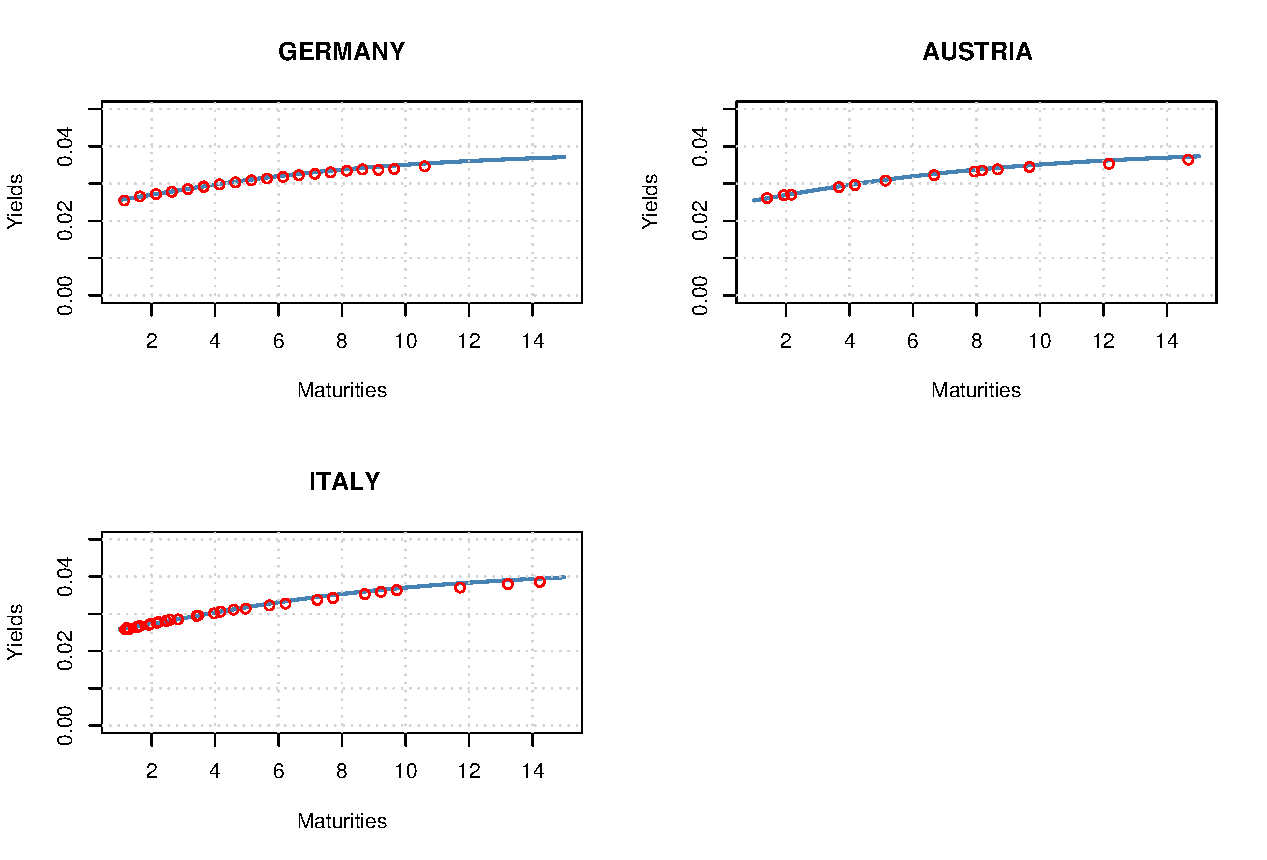
\includegraphics[width=1.0\textwidth]{pics/euro_nsg1.pdf}
	\caption{Zero-coupon yield curves}
\end{figure}

\begin{figure}[h]
\centering
	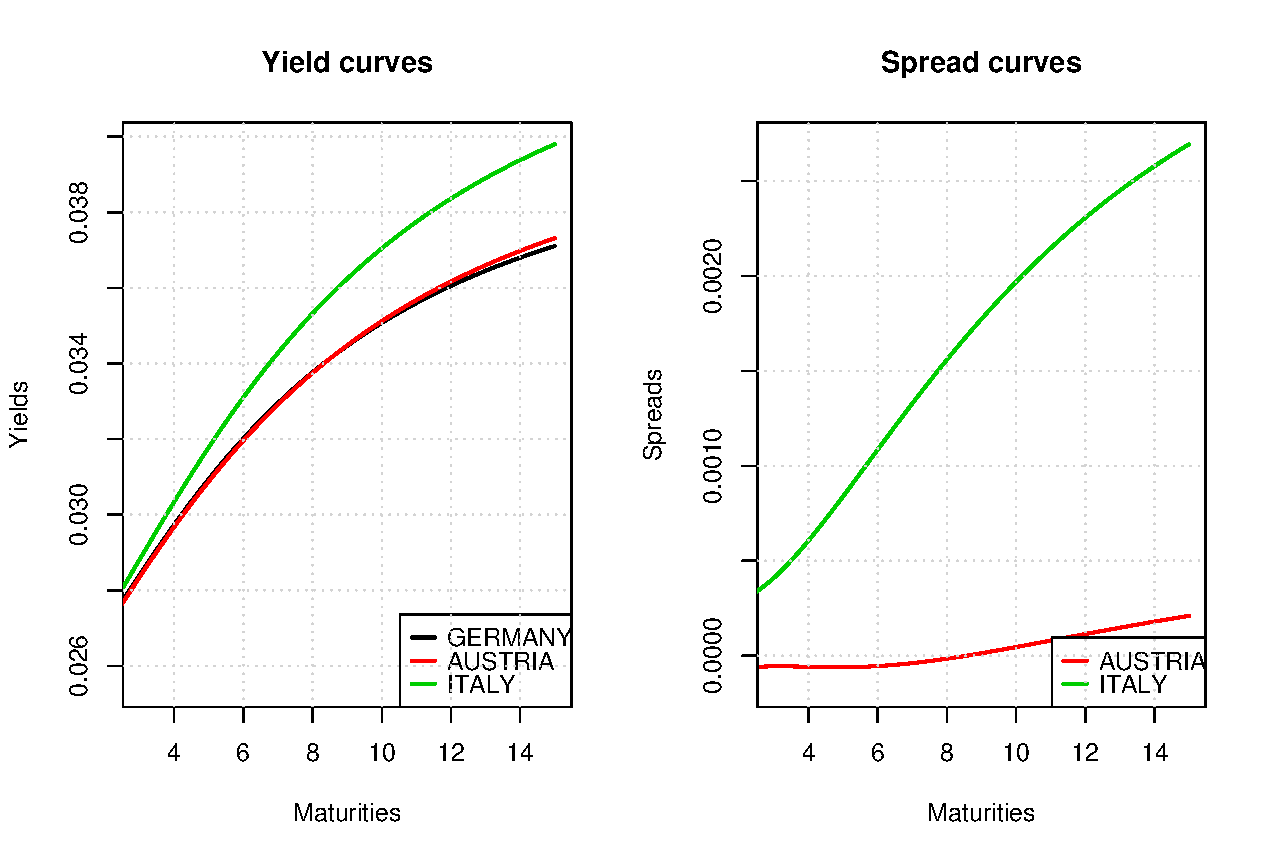
\includegraphics[width=1.0\textwidth]{pics/euro_nsg2.pdf}
	\caption{Spread curves }
\end{figure}

The presented example is easily accessible using the demo function in R. Use \newline
 \verb|demo(package="termstrc")| to explore the included demo examples.



 \section{Discussion}
 \section*{Acknowledgements}


 The authors are grateful to the students of the finance management science lab class of 2005.


%\nocite{*}
\listoftables
\listoffigures
\bibliographystyle{jss}
\bibliography{termstrc}


  \end{document} 